\documentclass[10pt,a4paper]{article} %#Establece el tipo de documento y sus especificaciones
%##Lista de paquetes que se podrán usar en el documento
\usepackage[left=2cm,right=2cm,top=2cm,bottom=2cm]{geometry}
\usepackage[dvipsnames]{xcolor}
\usepackage[fleqn]{mathtools}
\usepackage{booktabs}
\usepackage{amsmath}
\usepackage{latexsym}
\usepackage{graphicx}%##Paquete para llamar imagenes
\usepackage{nccmath}
\usepackage{multicol}
\usepackage{listings}
\usepackage{tasks}
\usepackage{color}
\usepackage{float}
\usepackage{lipsum}
\usepackage[spanish]{babel}
\UseRawInputEncoding

\definecolor{colorIPN}{rgb}{0.5, 0.0,0.13}
\definecolor{colorESCOM}{rgb}{0.0, 0.5,1.0}
\graphicspath{ {imagenes/} }

\begin{document} %##Indica donde inicia el documento
	%#########################################################
	\begin{titlepage}
		\centering
		{ \huge \bfseries \color{colorIPN}{Instituto Politécnico Nacional} \par}
		{ \Large \bfseries  \color{colorESCOM}{Escuela Superior de C{\' o}mputo} \par }
		\vspace{1cm}%##Inserta una separación de tamaño exacto entre líneas
		{\huge\Large \color{colorIPN}{Web App Development}.\par}
		\vspace{1.5cm}
		{\huge\Large  \color{colorESCOM}{Tarea 1 : Acceso a Datos con JDBC}\par}
		\vspace{2cm}
		{\Large\itshape \color{colorIPN}{Profesor: M. en C. Jos{\' e} Asunci{\' o}n Enr{\' i}quez Z{\' a}rate}\par} \hfill \break
		\vspace{2cm}
		{\Large\itshape \color{colorIPN}{Alumno: Mauro Sampayo Hern{\' a}ndez}\par} \hfill \break
		{\Large\itshape \color{colorIPN}{mauro\_luigi@hotmail.com}\par} \hfill \break
		{\Large\itshape \color{colorIPN}{3CM18} \par}
		\vfill
		{\large \color{colorIPN}{6 de septiembre de 2021}\par} 
		\vfill
	\end{titlepage}
	
	\renewcommand\lstlistingname{Quelltext} 
	
	\lstset{%##Formato para codigos SQL
		backgroundcolor=\color{white},
		basicstyle=\footnotesize,
		breakatwhitespace=false,
		breaklines=true,
		captionpos=b,
		commentstyle=\color{dkgreen},
		deletekeywords={...},
		escapeinside={\%*}{*)},
		extendedchars=true,
		frame=single,
		keepspaces=true,
		keywordstyle=\color{blue},
		language=SQL,
		morekeywords={*,modify,MODIFY,...},
		numbers=left,
		numbersep=15pt,
		numberstyle=\tiny,
		rulecolor=\color{gray},
		showspaces=false,
		showstringspaces=false, 
		showtabs=false,
		stepnumber=1,
		tabsize=4,
		title=\lstname
	}
	
	\settasks{
		counter-format=(tsk[r]),
		label-width=4ex
	}
	\tableofcontents 
	\pagebreak
	
	\pagenumbering {arabic} %##Coloca el contador de páginas a 1 y comienza a numerar de acuerdo con el estilo especificado. En este caso dicho estilo de numeracion es el arabigo
	
	\pagebreak
	
	%################################################
	\section{\color{colorIPN}{Introducci{\' o}n}}%##Crea secciones númeradas, en este caso esta es la seccion 1
	{\large En la actualidad, es casi indispensable realizar la clasificaci{\' o}n de datos de un sistema por medio de una base de datos. Sin embargo, a partir de esto surge la necesidad de llevar a cabo su correcta administraci{\' o}n al momento de recuperar o modificar los datos que se encuentren contenidos dentro de dicha base de datos, especialmente si se trata de una que se muy grande y compleja. 
		
		
		\vspace{0.5cm}
		Para satisfacer esta necesidad, hoy en d{\' i}a existen m{\' u}ltiples sistemas que se encargan de facilitar la administraci{\' o}n de los datos de las bases de datos, estos sistemas se conocen como Sistemas de Gesti{\' o}n de bases de datos (BDMS por sus siglas en ingl{\' e}s), los cuales se encarga de proveernos de mecanismos con los que se puedan llevar a cabo dichas tareas de manera sencilla.
		
		
		\vspace{0.5cm}
		Existe una gran cantidad de BDMS, sin embargo, para este reporte se har{\' a} {\' e}nfasis en las herramientas que provee SQL para la administraci{\' o}n de bases de datos y la API JDBMS que brinda la posibilidad de realizar conexiones a bases de datos desde una aplicaci{\' o}n de Java, y a partir de esta poder realizar modificaciones en las mismas.}
	
	%\subsection{ \color{colorESCOM}{Sub Sección 1}} %##Crea subsecciones numeradas
	%\lipsum[2-3] %##Añade tecto lorem ipsum
	
	\pagebreak
	
	%################################################
	\section{\color{colorIPN}{Conceptos}}
	{\large A continuaci{\' o}n se enlista una serie de conceptos, que son necesarios para poder entender m{\' a}s a detalle la funcionalidad de una Base de Datos y los Sistemas de Gesti{\' o}n que las administran}
	
	\subsection{ \color{colorESCOM}{SQL}}
	{\large SQL es un lenguaje est{\' a}ndar internacional que hace uso de bases de datos relacionales para realizar queries (aquellos que realizan la solicitud de informaci{\' o}n que satisfaga ciertos criterios) y la manipulaci{\' o}n de datos.}
	
	\subsection{ \color{colorESCOM}{Base de Datos Relacional}}
	{\large Una base de datos relacional es una representaci{\' o}n l{\' o}gica de datos que permiten acceso a los datos sin considerar su estructura f{\' i}sica.}
	
	\subsection{ \color{colorESCOM}{Sistemas de Gesti{\' o}n de Bases de Datos (BDMS)}}
	{\large Un Sistema de Gesti{\' o}n de bases de datos (BDMS por sus siglas en ingl{\' e}s) es un sistema que provee mecanismos para el almacenamiento, organizaci{\' o}n, recuperaci{\' o}n y modificaci{\' o}n de datos por distintos usuarios sin afectar la representaci{\' o}n interna de los datos.}
	
	\subsection{ \color{colorESCOM}{Statement(sentencia)}}
	{\large Es una herramienta que sirve para procesar una sentencia SQL est{\' a}tica y obtener los resultados producidos por ella.}
	
	\pagebreak
	
	%################################################
	\section{\color{colorIPN}{Desarrollo}}
	{\large Una base de datos relacional es una representaci{\' o}n l{\' o}gica de datos que permiten acceso a los datos sin consideraci{\' o}n de su estructura f{\' i}sica, y almacena dichos datos en tablas. En la figura \ref{img1} se muestra un ejemplo de base de datos relacional; en este caso el nombre de la tabla es \textbf{Employee}, y su prop{\' o}sito es el de almacenar los atributos de los empleados.}
	
	\begin{figure}[H]\label{img1}
		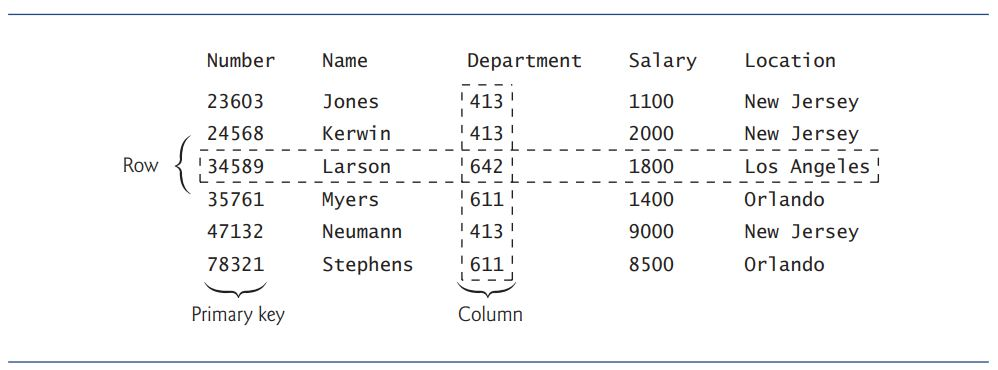
\includegraphics[width=0.8\textwidth]{Figura1.jpg}
		\centering
		\label{img:Figura1}
	\end{figure}
	
	Las tablas se componen de filas y columnas en las cuales se almacenan los valores de la tabla. En el caso de la tabla de la Figura 1 se tienen seis filas. La columna \textbf{Number} dé cada fila es la clave primaria o primary key, que es aquella columna que contiene un {\' u}nico valor por cada fila, y el cu{\' a}l no puede ser duplicado, asegurando as{\' i} que cada fila puede ser identificada por su clave primaria. Algunos ejemplos de llaves primaria son los n{\' u}meros de seguridad social, los IDs de empleado, etc. Las filas de una tabla pueden ser ordenadas en un orden en especifico o no tener ning{\' u}n orden en particular
	
	%######################################################
	
	\subsection{\color{colorESCOM}{Manipulaci{\' o}n de datos con SQL}}
	{\large Uno de los Sistema de Gesti{\' o}n de bases de datos m{\' a}s utilizados en la actualidad es SQL, el cual nos permite realizar la consulta y modificaci{\' o}n de datos de tablas en una Base de Datos por medio de cl{\' a}usulas. A continuaci{\' o}n, se describen las cl{\' a}usulas m{\' a}s importantes para la consulta y modificaci{\' o}n de datos de una base de datos en SQL.
	}
	
	\subsubsection{\color{colorESCOM}{Clausula SELECT…FROM}}
	{\large Realiza la recuperaci{\' o}n de datos de una o m{\' a}s tablas, seleccionando aquellas columnas de las tablas de una base de datos que sean requeridas. La forma b{\' a}sica de esta consulta es:
		
		\begin{lstlisting}
			SELECT * FROM nombreTabla
		\end{lstlisting}
		
		Donde el asterisco (*) indica que todas las columnas de la tabla \textit{nombreTabla} deben ser recuperadas. Para realizar la recuperaci{\' o}n de solo ciertas columnas de la tabla, se debe remplazar el asterisco (*) con la lista de columnas que se deseen consultar separadas por una coma (,).
		
		
		\begin{lstlisting}
			SELECT nombreCulumna1, nombreColumna2,… FROM nombreTabla.
		\end{lstlisting}
	}
	
	\subsubsection{\color{colorESCOM}{Clausula WHERE}}
	{\large Indica el criterio de selecci{\' o}n que determinar{\' a} que filas de una tabla ser{\' a}n recuperadas, eliminadas o actualizadas durante una consulta. La forma b{\' a}sica de esta consulta es:
		
		\begin{lstlisting}
			SELECT nombreCulumna1, nombreColumna2,…
			FROM nombreTabla.
			WHERE criterioSeleccion.
		\end{lstlisting}
		
		La cl{\' a}usula WHERE puede hacer uso de los operadores $<$, $>$, \leq, \geq, <> y \textit{LIKE}. 
		
		
		\vspace{0.5cm}
		El operador \textit{LIKE} es usado para realizar la b{\' u}squeda de cadenas de texto que coincidan o cumplan con un determinado patr{\' o}n. El operador \textit{LIKE} se auxilia de los caracteres de porcentaje (\%) y gu{\' i}{\' o}n bajo (\_).
		
		
		\vspace{0.5cm}
		El caracter de porcentaje (\%) realizara la b{\' u}squeda de cadenas de texto que tengan cero o m{\' a}s caracteres desde la posici{\' o}n del caracter de porcentaje (\%), mientras que el car{\' a}cter guion bajo (\_) indica que puede haber cualquier caracter en dicha posici{\' o}n. Por ejemplo:
		
		\begin{lstlisting}
			SELECT ColumnaA, ColumnaB,…
			FROM Tabla.
			WHERE ColumnaA LIKE ‘_o%z’
		\end{lstlisting}
		
		En este ejemplo a consulta seleccionar{\' a} {\' u}nicamente las filas que cumplan con la condici{\' o}n, de que en la Columna B haya una cadena de texto que cumpla con el siguiente patr{\' o}n: Que inicie con cualquier car{\' a}cter que sea seguido de una `o’, posteriormente haya de o a m{\' a}s caracteres que finalicen con `z’. Cabe destacar que los patrones de b{\' u}squeda siempre deben estar escritos entre comillas simples (`’).
	}
	
	\subsubsection{\color{colorESCOM}{Clausula ORDER BY}}
	{\large Indica los criterios a seguir para realizar el ordenamiento de filas de una tabla. Las filas pueden ser ordenadas de manera ascendente o descendente. . La forma b{\' a}sica de esta consulta es:
		
		\begin{lstlisting}
			SELECT ColumnaA, ColumnaB,…  FROM nombreTabla.  ORBER BY ColumnaA ASC
			SELECT ColumnaA, ColumnaB,…  FROM nombreTabla.  ORBER BY ColumnaA DESC
		\end{lstlisting}
		
		Donde ASC especifica un ordenamiento de forma ascendente (del menor al mayor valor), y DESC ordenamiento de forma descendente (del mayor al menor valor). En caso de no especificar el tipo de ordenamiento en la cl{\' a}usula ORDER BY, este se realizar{\' a} de forma ascendente por defecto. 
		
		
		\vspace{0.5cm}
		La cl{\' a}usula ORDER BY puede ser usada junto a la cl{\' a}usula WHERE y puede realizar el ordenamiento usando de referencia m{\' a}s de una columna, sin necesidad de que estas deban tener el mismo tipo de ordenamiento.}
	
	\subsubsection{\color{colorESCOM}{Clausula INNER JOIN}}
	{\large Realiza la uni{\' o}n de filas de m{\' u}ltiples tablas que conforman una base de datos en una sola. La forma b{\' a}sica de esta consulta es:
		
		\begin{lstlisting}
			SELECT columna1, columna2,…
			FROM tabla1.
			INNER JOIN tabla2
			ON tabla1.columna = table 2.columa
		\end{lstlisting}
		
		La cl{\' a}usula ON especifica las columnas de cada tabla, que tendr{\' a}n que ser comparadas para determinar que filas ser{\' a}n unidas. Cabe destacar que la utilizaci{\' o}n del punto (.) en las columnas de la tabla, se realiza para indicar a que tabla pertenece cada columna dado el caso de que haya dos columnas con el mismo nombre en dos tablas distintas.}
	
	\subsubsection{\color{colorESCOM}{Clausula INSERT}}
	{\large Realiza la inserci{\' o}n de filas en una tabla especifica.  La forma b{\' a}sica de esta consulta es:
		
		\begin{lstlisting}
			INSERT INTO nombreTabla (columna1, clumna2,…,columnaN)
			VALUES (valor1, valor2, …, valorN)
		\end{lstlisting}
		
		Donde \textit{nombreTabla} es la tabla donde se insertar{\' a} la fila y que estar{\' a} seguida por una lista de elementos separada por comas y entre paréntesis, especificando las columnas donde ser{\' a}n insertados los datos. Posteriormente se coloca la clausula VALUES seguida por una lista de elementos separada por comas y entre paréntesis, con los valores a insertar en cada una de las columnas especificadas anteriormente, los cuales deben coincidir con el tipo de dato especificado para cada columna.}
	
	\subsubsection{\color{colorESCOM}{Clausula UPDATE}}
	{\large Realiza la actualizaci{\' o}n y modificaci{\' o}n de filas en una tabla especifica.  La forma b{\' a}sica de esta consulta es:
		
		\begin{lstlisting}
			UPDATE nombreTabla
			SET columna1 = valor1, columna2 = valor2, …, columnaN = valorN
			WHERE   criterioSeleccion
		\end{lstlisting}
		
		Donde \textit{nombreTabla} es la tabla por actualizar, seguido de la cl{\' a}usula SET y una lista separada por comas, con el formato \textit{nombreColumna = valor}. La cl{\' a}usula WHERE es opcional y provee de un criterio de selecci{\' o}n que ayuda a determinar que filas ser{\' a}n actualizadas.}
	
	\subsubsection{\color{colorESCOM}{Clausula DELETE}}
	{\large Realiza la eliminaci{\' o}n de filas en una tabla especifica.  La forma b{\' a}sica de esta consulta es:
		
		\begin{lstlisting}
			DELETE FROM nombreTabla  WHERE criterioSeleccion
		\end{lstlisting}
		
		Donde \textit{nombreTabla} es la tabla en donde se realizar{\' a} la eliminaci{\' o}n. La cl{\' a}usula WHERE es opcional y provee de un criterio de selecci{\' o}n que ayude a determinar que filas ser{\' a}n eliminadas.}
	
	%####################################################################
	\subsection{\color{colorESCOM}{Manipulaci{\' o}n de datos con la API JDBC}}
	{\large La API JDBC es una API de Java muy {\' u}til, que permite la conexi{\' o}n y el acceso a una base de datos desde una aplicaci{\' o}n Java, para poder manipular y consultar la informaci{\' o}n contenida en estas desde la misma aplicaci{\' o}n.
	}
	
	\subsubsection{\color{colorESCOM}{Conexi{\' o}n a una base de datos por medio de la API JDBC}}
	{\large A continuaci{\' o}n, se explican los pasos generales para realizar la conexi{\' o}n a una base de datos desde una aplicaci{\' o}n Java por medio de la API JDBC.
		
		\begin{enumerate}       
			{\large     
				\item Se importan las interfaces JDBC y las clases del paquete java.sql, las cu{\' a}les contienen todas las clases y métodos necesarios para realizar la conexi{\' o}n a la base de datos desde la aplicaci{\' o}n Java, y la manipulaci{\' o}n de datos de esta.
				\item Se declara una cadena de texto que contiene el URL de la base de datos, la cual servir{\' a} como identificaci{\' o}n de la base de datos a la cual se realizar{\' a} la conexi{\' o}n. La URL debe tener el siguiente formato: 
				
				\underline{protocoloComunicacion: subprotocoloComunicacion l://localizacionBD/nombreBD }
				\item En el método main se crea un objeto de tipo \textit{Connection}, el cu{\' a}l administrar{\' a} la conexi{\' o}n ente el programa en Java y la base de datos. 
				\item Se inicializa la conexi{\' o}n llamando al método \textit{getConnection} de la clase \textit{DriveManager }, que intentar{\' a} realizar la conexi{\' o}n con la base de datos especificada en la URL. Este método recibe 3 atributos tipo string; en el primer atributo se debe ingresar la URL de la base de datos a acceder, en el segundo el usuario y en el tercero la contrase{\~n}a del usuario.
			}
		\end{enumerate}
		
		De esta manera nuestra aplicaci{\' o}n de Java se conectar{\' a} exitosamente a la base de datos.
	}
	
	\subsubsection{\color{colorESCOM}{Manipulaci{\' o}n y consulta de datos por medio de la API JDBC}}
	{\large A continuaci{\' o}n, se explican los pasos generales para realizar la manipulaci{\' o}n de datos utilizando cl{\' a}usulas de SQL, desde una aplicaci{\' o}n Java por medio de la API JDBC.
		
		\begin{enumerate}       
			{     
				\item Se invoca el método \textit{createStatement} de la clase \textit{Connection} para la creaci{\' o}n de un statement de SQL, el resultado de dicho método se guardar{\' a} en un objeto tipo \textit{Statement}.
				\item Se invoca el método \textit{executeQuery} de la clase \textit{Statement}, que recibir{\' a} un atributo de tipo string, donde se ingresar{\' a} el statement de SQL, que contendr{\' a} la instrucci{\' o}n de consulta o modificaci{\' o}n de datos que se desee realizar. Esté método se encargar{\' a} de realizar la acci{\' o}n correspondiente a dicho statement y guardar{\' a} la informaci{\' o}n resultante en un objeto de tipo ResultSet.
				\item Se obtiene la metadata de los resultados del statement, almacenados previamente en el objeto de tipo \textit{ResultSet}, por medio del método \textit{getColumnCount} de la clase \textit{ResultSertMetaData}.
				\item Si se desea imprimir los datos de la base de datos para poder visualizar la consulta o modificaci{\' o}n realizados sobre esta, se puede hacer lo siguiente:
				
				\begin{enumerate}       
					{    
						\item Por medio del método \textit{getColumnName} de la clase \textit{ResultSertMetaData} y con ayuda de un ciclo for se pueden imprimir los nombres de todas las columnas que conforman la tabla, utilizando la metadata de los resultados de la consulta realizada previamente.
						\item Por medio del método \textit{getObject} de la clase \textit{ResultSet} y con ayuda de un ciclo for se pueden imprimir la informaci{\' o}n que contienen las filas de la columna de la tabla.
					}
				\end{enumerate}
				
				\item  Finalmente, y una vez finalizada la manipulaci{\' o}n y consulta de datos, dentro de un bloque finally se realiza el cierre de los objetos de tipo \textit{ResultSet}, \textit{Statement} y \textit{Connection}.   
			}
		\end{enumerate}
	}
	
	%####################################################################
	
	\subsection{\color{colorESCOM}{PreparedStatements}}
	{\large Un PreparedStatemente es una herramienta que permite la creaci{\' o}n de statements SQL que permiten la ejecuci{\' o}n de del mismo query repetidamente con diferentes valores en sus par{\' a}metros. A diferencia de los Statements normales, estos est{\' a}n parametrizados de tal forma que resultan tener mayor eficiencia que los Statements.
		
		
		\vspace{0.5cm}
		A continuaci{\' o}n, se presenta un ejemplo de un PreparedStatement implementado en Java por medio de la clase \textit{PreparedStatements}:
		
		\begin{figure}[H]
			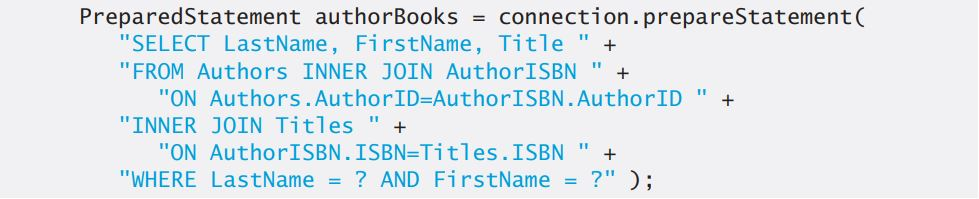
\includegraphics[width=\textwidth]{Figura2.jpg}
			\centering
			\caption{Ejemplo de un \textit{PreparedStatement}}
			\label{img:Figura2}
		\end{figure}
		
		Los dos signos de interrogaci{\' o}n (?) representan placeholders, en donde se podr{\' a}n colocar valores que pasar{\' a}n a ser parte del query se realice en la base de datos. Para poder colocar dichos valores se tiene que recurrir al método \textit{setString} de la clase \textit{PreparedStatements} como se muestra a continuaci{\' o}n:
		
		\begin{figure}[H]
			
\includegraphics[width=\textwidth]{Figura3.jpg}
			\centering
			\caption{Ejemplo método \textit{setString} de la clase \textit{PreparedStatement}}
			\label{img:Figura3}
		\end{figure}
		
		El método \textit{setString} como se puede observar recibe dos argumentos. El primero representa el n{\' u}mero de par{\' a}metro en donde se colocar{\' a} el valor en cuesti{\' o}n (la numeraci{\' o}n de los par{\' a}metros inicia siempre en 1, empezando desde el primer signo de interrogaci{\' o}n (?) que haya sido colocado); y el segundo representa el valor que se colocar{\' a} en el par{\' a}metro.
	}
	
	\pagebreak
	
	%################################################
	\section{\color{colorIPN}{Resultados}}
	{\large Tras finalizar la revisi{\' o}n del documento, se logr{\' o} el entendimiento acerca de que es un Sistema de Gesti{\' o}n de Bases de Datos, la identificaci{\' o}n de las instrucciones para manipular datos en bases de datos por medio de SQL y sus respectivas funciones y el funcionamiento de la API JDBC.
		
		
		\vspace{0.5cm}
		De igual manera se logr{\' o} el entendimiento de todos los pasos a seguir para realizar una aplicaci{\' o}n en Java que pueda acceder a Bases de Datos por medio de JDBC.}
	
	\pagebreak
	
	
	%################################################
	\section{\color{colorIPN}{Conclusi{\' o}n}}
	{\large El uso de Sistemas de Gesti{\' o}n para la administraci{\' o}n, ordenamiento y modificaci{\' o}n de datos de las tablas de una base de datos es de vital importancia para el correcto funcionamiento de un sistema, pues estas son necesarias para llevar a cabo la manipulaci{\' o}n de los datos de manera eficaz, segura y sencilla. 
		
		
		\vspace{0.5cm}
		De igual forma las herramientas que nos provee JDBC y SQL resultan muy {\' u}tiles al momento de llevar a cabo el proceso anteriormente mencionado, en especial al momento de desarrollar aplicaciones en Java que se conecten con una base de datos para manipularla.}
	
	\color{colorIPN}{
		\begin{flushright}
			\textit{
				Mauro Sampayo Hern{\' a}ndez
			}
		\end{flushright} \hfill \break
	}
	
	\pagebreak
	
	%################################################
	
	\section{\color{colorIPN}{Referencias Bibliogr{\'a}ficas}}
	\color{colorESCOM}{
		\begin{thebibliography}{10}
			\bibitem{JDBC}
			\newblock {\em Chapter 28. Accesing Databases with JDBC}
		\end{thebibliography}
	}
	
\end{document} %##Indica donde termina el documento
